% !TeX program = pdflatex
% !TeX encoding = utf8
% !TeX spellcheck = uk_UA
% !BIB program = bibtex8

\documentclass[18pt]{LectMechanics}
\usetikzlibrary{patterns, snakes, intersections}
\tikzset{
	body/.pic = {
			\fill[red!40, draw=red, opacity=0.5]  plot[smooth cycle, tension=.7] coordinates {
			(-2.5,0.5)
			(-0.5,2.5)
			(1.5,2)
			(2,0.5)
			(1,-1.5)
			(-1.5,-1.5)
		};
	}
}



\usetikzlibrary{arrows.meta}

\title[Physics 1]{\huge\bfseries Work and energy}
\date{}

\begin{document}
%=======================================================================================================
%\usebackgroundtemplate{
%
%\tikz\node[opacity=0.3]{\includegraphics[width=\paperwidth,height=\paperheight]{background}};%
%}
\begin{frame}
	\titlepage
\end{frame}
%=======================================================================================================
\usebackgroundtemplate{
}




%=======================================================================================================
\begin{frame}{Goals for Lecture}{}
	\begin{itemize}
		\item To understand and calculate the work done by a force.
		\item To understand the meaning of kinetic energy.
		\item To learn how work changes the kinetic energy of a body and how to use this principle.
		\item To relate work and kinetic energy when the forces are not constant or the body follows a curved path.
		\item To solve problems involving power.
	\end{itemize}
\end{frame}
%=======================================================================================================

%=======================================================================================================
\begin{frame}{Work Done by a Constant Force}{}
	\begin{columns}
		\begin{column}{0.6\linewidth}
			The work $W$ done on a system by an agent exerting a constant force on the
			system is the product of the magnitude $F$ of the force, the magnitude $\Delta r$ of
			the displacement of the point of application of the force, and $\cos\alpha$, where $\alpha$ is
			the angle between the force and displacement vectors:
			\begin{equation*}
				W = F\Delta r \cos\alpha
			\end{equation*}
			Or using definition of scalar product of two vectors:
			\begin{equation*}
				W = \vec F \cdot \Delta\vec r
			\end{equation*}
			\begin{center}
				\textcolor{red}{Work $W$ is the SCALAR quantity!}
			\end{center}
		\end{column}
		\begin{column}{0.4\linewidth}
			\begin{center}
				\begin{tikzpicture}
					\pgfmathsetmacro{\ang}{30}
					\draw[gray!80!black, ultra thick] (-2,0) -- (2,0);
					\fill[top color = gray, bottom color = white] (-2,-0.25) rectangle (2,0);
					\draw[brown, ultra thick, fill=brown!50] (-1.5,0) rectangle +(1,1) [add reference=B1];
					\draw[opacity=0.2, brown, ultra thick, fill=brown!50] (0.5,0) rectangle +(1,1) [add reference=B2];
					\foreach \i in {1,2} {
							\draw (B\i\space  center) -- +(0,-1) coordinate (A\i);
							\draw[-latex, ultra thick, red] (B\i\space  center) -- +(\ang:1.5) node[above] {$\vec F$};}
					\draw[dashed] (B1 center) -- +(1,0);
					\draw (B1 center) +(0:0.6) arc (0:\ang:0.6) node[right, pos=0.5] {$\alpha$};
					\draw[-latex, ultra thick] (A1) -- node[below] {$\Delta \vec r$}(A2);
				\end{tikzpicture}
			\end{center}
		\end{column}
	\end{columns}
\end{frame}
%=======================================================================================================

%=======================================================================================================
\begin{frame}{Work Done by a Varying Force}{}
	\begin{columns}
		\begin{column}[T]{0.7\linewidth}\small
			\only<1>{
				Consider a particle being displaced along the $x$ axis under the action of a force that
				varies with position. The particle is displaced in the direction of increasing $x$ from
				$x = x_i$ to $x = x_f$. In such a situation, we cannot use $W = F\Delta r \cos\alpha$ to calculate the
				work done by the force because this relationship applies only when $\vec F$ is constant
				in magnitude and direction. If, however, we imagine that the particle undergoes a
				very small displacement $dx$, the $x$ component $F_x$ of
				the force is approximately constant over this small interval; for this small displacement,
				we can approximate the work done on the particle by the force as
				\begin{equation*}
					\delta W \approx F_x \Delta x
				\end{equation*}
				which is the area of the shaded rectangle.
			}
			\only<2>{
				If we imagine the $F_x$ versus
				$x$ curve divided into a large number of such intervals, the total work done for the
				displacement from $x_i$ to $x_f$ is approximately equal to the sum of a large number of such terms:
				\begin{equation*}
					W \approx \sum\limits_{x_i}^{x_f} F_x \Delta x
				\end{equation*}
				If the size of the small displacements is allowed to approach zero, the number of
				terms in the sum increases without limit but the value of the sum approaches a definite
				value equal to the area bounded by the $F_x$ curve and the $x$ axis:
				\begin{equation*}
					W = \lim\limits_{\Delta x\to 0} \sum\limits_{x_i}^{x_f} F_x \Delta x = \int\limits_{x_i}^{x_f} F_x dx
				\end{equation*}
			}
			\only<3>{
				For the general case of a net force $\vec F$ whose magnitude and direction may vary, we use the scalar product:
				\begin{equation*}
					\tcbhighmath[drop fuzzy shadow]{W = \int\limits_\mathrm{point\, 1}^\mathrm{point\, 2} \vec F d\vec r = \int\limits_\mathrm{point\, 1}^\mathrm{point\, 2} F_x dx + F_y dy + F_z}
				\end{equation*}
				where integration done between point 1 and point 2 of the body trajectory.
				\begin{center}
					\begin{tikzpicture}
						\draw [thick, brown,
							tangent=0.1,
							tangent=0.3,
							tangent=0.6,
							tangent=0.9,
							decoration={markings,
									mark=at position 0.5 with \arrow{latex},
									mark=at position 0.1 with {
											\coordinate (P1);
											\node[below, black] at (P1) {$P_1$};
											\fill[red!50] circle [radius=2pt];
										},
									mark=at position 0.9 with {
											\coordinate (P2);
											\node[below, black] at (P2) {$P_2$};
											\fill[red, red!50] circle [radius=2pt];
										},
								},
							postaction=decorate] (0,0) .. controls (3,1) and (3,-2).. (6,0);
						\foreach \i in {1,2,3,4} {
								\draw[-latex, blue, thick, use tangent=\i] (0,0) -- (0.5,0) node[above] {$d \vec r$};
								\draw[-latex, red, thick, use tangent=\i] (0,0) -- ({50+20*\i}:1) node[above] {$\vec F$};
							}
					\end{tikzpicture}
				\end{center}
			}
		\end{column}
		\begin{column}[T]{0.3\linewidth}
			\vspace{-20pt}%
			\begin{center}
				\includegraphics[height=0.85\textheight]{Work}
			\end{center}
		\end{column}
	\end{columns}
\end{frame}
%=======================================================================================================

%=======================================================================================================
\begin{frame}{Power}{}
	To characterize intensity of the work performed, the quantity called \emph{power} is introduced. Power is denned as the work performed by a force per unit time:
	\begin{equation*}
		\tcbhighmath[drop fuzzy shadow]{N = \frac{dW}{dt}.}
	\end{equation*}
	If the force $\vec F$ performs the work $ \vec F \cdot d\vec r$ during the time interval $dt$, the power developed by that force at a given moment of time is equal to $N = \vec F \cdot \frac{d\vec r}{dt}$; taking into account that $\frac{d\vec r}{dt} = \vec v$, we obtain
	\begin{equation*}
		N = \vec F \cdot \vec v.
	\end{equation*}
	Thus, the power developed by the force $ \vec F $ is equal to the scalar product of the force vector by the vector of velocity $ \vec v $ with which the point moves under the action of the given force. Just like work, power is an scalar quantity.

\end{frame}
%=======================================================================================================

%=======================================================================================================
\begin{frame}{Kinetic energy}{}
	\begin{enumerate}
		\item The kinetic energy of a particle is \emph{$K = \frac{mv^2}{2}$}.
		\item The net work on a body changes its velocity and therefore its kinetic energy.
		      \begin{center}
			      \begin{tikzpicture}
				      \pgfmathsetmacro{\ang}{30}
				      \draw[gray!80!black, ultra thick] (-5,0) -- (5,0);
				      \fill[top color = gray, bottom color = white] (-5,-0.25) rectangle (5,0);
				      \draw[brown, ultra thick, fill=brown!50] (-4.5,0) rectangle +(1,1) [add reference=B1];
				      \draw[opacity=0.5, brown, ultra thick, fill=brown!50] (2.5,0) rectangle +(1,1) [add reference=B2];
				      \node[above] at (B1 north) {$K_\mathrm{initial} = \frac{mv^2_\mathrm{initial}}{2}$};
				      \draw[-latex, red, ultra thick] (B1 east) -- +(2,0) node[right] {$\vec v_\mathrm{initial}$};
				      \node[above] at (B2 north) {$K_\mathrm{final} = \frac{mv^2_\mathrm{final}}{2}$};
				      \draw[-latex, red, ultra thick] (B2 east) -- +(1,0) node[right] {$\vec v_\mathrm{final}$};
			      \end{tikzpicture}
		      \end{center}
		\item The work-energy theorem: The work done by the net force on a particle equals the change in the particle's kinetic energy.

		      Mathematically, the \emph{Work-kinetic energy theorem} is expressed as:
		      \begin{equation*}
			      \tcbhighmath[drop fuzzy shadow]{W = K_\mathrm{final} - K_\mathrm{initial}.}
		      \end{equation*}
	\end{enumerate}
\end{frame}
%=======================================================================================================

%=======================================================================================================
\begin{frame}{Potential Energy}{}
	One job of physics is to identify the different types of energy in the world, especially those that are of common importance. One general type of energy is \emph{potential energy $U$}.Technically, potential energy is energy that can be associated with the configuration (arrangement) of a system of objects that exert forces on one another.
	%---------------------------------------------------------
	\begin{minipage}{0.6\linewidth}
		\only<1>{\small%
			The system of objects consists of Earth and the Asteroid. The force between the objects is the gravitational force. The configuration of the system changes (the separation between the Asteroid and Earth changes). We can account for the Asteroid's motion and increase in kinetic energy by defining a gravitational potential energy $U$.This is the energy associated with the state of separation between two objects that attract each other by the gravitational force.
		}
		\only<2>{%
			For either rise or fall, the change \[\Delta U = U_2 - U_1\] in gravitational potential energy is defined as being equal to the negative of the work done on the Asteroid by the gravitational force:
			\begin{equation*}
				\tcbhighmath[drop fuzzy shadow]{W = -\Delta U}
			\end{equation*}
		}
	\end{minipage}%
	%---------------------------------------------------------
	\begin{minipage}{0.4\linewidth}\centering
		\begin{overprint}
			\begin{tikzpicture}
				\pgfmathsetmacro{\ang}{45}
				\coordinate (B1) at (0,0);
				\coordinate (B2) at (\ang:5);
				%\pgfextractangle{\bangle}{(B1)}{(B2)}
				\draw[-latex, red, double] (B1) -- ($(B1)!1cm!(B2)$);
				\draw[-latex, blue, double] (B2) -- ($(B2)!1cm!(B1)$);
				\draw[ball color=blue] (B1) circle (0.6);
				\draw[ball color=red] (B2) circle (0.2);
				\foreach \i in {0.5,1,2,3.5} {
						\draw[ball color=red, opacity=0.3] ([shift={(180+\ang:\i)}]B2) circle (0.2);
					}
				\draw[dashed] (B1) -- (B2) node[below, pos=0.5] {$r$};
				\node[below=1cm] at (B1) {Earth};
				\node[below=1cm] at (B2) {Asteroid};
			\end{tikzpicture}
		\end{overprint}
	\end{minipage}
	%---------------------------------------------------------
\end{frame}

%=======================================================================================================
\begin{frame}{Conservative and Nonconservative Forces}{}
	\begin{enumerate}
		\item When the system configuration changes, the force does work (call it $W_1$) on the body, transferring energy between the kinetic energy $K$ of the body and some other type of energy of the system.
		\item  When the configuration change is reversed, the force reverses the energy 	transfer, doing work $W_2$ in the process.
	\end{enumerate}
	%---------------------------------------------------------
	\begin{minipage}{0.5\linewidth}
		In a situation in which $W_1 = -W_2$ is always true, the other type of energy is a potential energy and the force is said to be a \emph{conservative force.} The gravitational force conservative.
	\end{minipage}%
	%---------------------------------------------------------
	\begin{minipage}{0.5\linewidth}\centering
		\begin{center}
			\includegraphics[width=0.5\linewidth]{UpDownBody}
		\end{center}
	\end{minipage}
	%---------------------------------------------------------
	Forces for which this ratio is not satisfied are called a \emph{nonconservative force}. The frictional force is nonconservative.
\end{frame}
%=======================================================================================================

%=======================================================================================================
\begin{frame}{Path Independence of Conservative Forces}{}
	The primary test for determining whether a force is conservative or nonconservative is this:
	%---------------------------------------------------------
	\begin{minipage}{0.5\linewidth}
		Any choice of path between the points gives the same amount of work:
		\begin{equation*}
			W_\mathrm{A \to B \, by\, path\, 1} = W_\mathrm{A \to B \, by\, path\, 2}
		\end{equation*}
	\end{minipage}%
	%---------------------------------------------------------
	\begin{minipage}{0.5\linewidth}\centering
		\begin{center}
			\begin{tikzpicture}
				\coordinate (A) at (0,0);
				\coordinate (B) at (2,2);
				\draw[red!50, ultra thick,
					decoration={markings, mark=at position 0.5 with
							\arrow{latex}
							\node[above] {$1$};
						},
					postaction=decorate,
				] (A) to[in=180, out=90] (B);

				\draw[blue!50, ultra thick,
					decoration={markings, mark=at position 0.5 with
							\arrow{latex}
							\node[below] {$2$};
						},
					postaction=decorate,
				] (A) to[in=-90, out=0] (B);
				\node[pt=red] at (A) {}; \node[below left] at (A) {$A$};
				\node[pt=blue] at (B) {};\node[below right] at (B) {$B$};
			\end{tikzpicture}
		\end{center}
	\end{minipage}
	%---------------------------------------------------------

	%---------------------------------------------------------
	\begin{minipage}{0.5\linewidth}
		A round trip gives a total work
		of zero:
		\begin{equation*}
			W_\mathrm{A \to B \, by\, path\, 1} + W_\mathrm{B \to A \, by\, path\, 2} = 0
		\end{equation*}
	\end{minipage}%
	%---------------------------------------------------------
	\begin{minipage}{0.5\linewidth}\centering
		\begin{center}
			\begin{tikzpicture}
				\coordinate (A) at (0,0);
				\coordinate (B) at (2,2);
				\draw[red!50, ultra thick,
					decoration={markings, mark=at position 0.5 with
							\arrow{latex}
							\node[above] {$1$};
						},
					postaction=decorate,
				] (A) to[in=180, out=90] (B);

				\draw[blue!50, ultra thick,
					decoration={markings, mark=at position 0.5 with
							\arrow{latex}
							\node[below] {$2$};
						},
					postaction=decorate,
				] (B) to[in=0, out=-90] (A);
				\node[pt=red] at (A) {}; \node[below left] at (A) {$A$};
				\node[pt=blue] at (B) {};\node[below right] at (B) {$B$};
			\end{tikzpicture}
		\end{center}
	\end{minipage}
	%---------------------------------------------------------
	\begin{boxedframe}
		The net work done by a conservative force on a particle moving around any closed path is zero.
	\end{boxedframe}
\end{frame}
%=======================================================================================================

%=======================================================================================================
\begin{frame}{Path Independence of Conservative Forces}{An example}
	A block of cheese slides along a frictionless track
	from point a to point b. (b) Finding the work done on the cheese by
	the gravitational force is easier along the dashed path than along
	the actual path taken by the cheese; the result is the same for
	both paths.
	\begin{center}
		\includegraphics[width=0.7\linewidth]{PathIndependentWork}
	\end{center}
\end{frame}
%=======================================================================================================

%=======================================================================================================
\begin{frame}{Determining Potential Energy Values}{}
	When that force does work $W$ on the body, the change $\Delta U$ in
	the potential energy associated with the system is the negative of the work done:
	\begin{equation*}
		\tcbhighmath[drop fuzzy shadow]{W = -\Delta U}
	\end{equation*}

	\begin{boxedframe}
		Thus, for calculating the value of potential energy we need to calculate the work of force work $W$ on the body.
	\end{boxedframe}

\end{frame}
%=======================================================================================================

%=======================================================================================================
\begin{frame}{Gravitational Potential Energy}{}
	%---------------------------------------------------------
	\begin{minipage}{0.7\linewidth}
		We first consider a particle with mass m moving vertically along a $y$ axis (the positive direction is upward). As the particle moves from point $y_i$ to point $y_f$ , the gravitational force does work on it.To find the corresponding change in the gravitational potential energy of the particle–Earth system, we use $W = -\Delta U$ with two changes:
	\end{minipage}%
	%---------------------------------------------------------
	\begin{minipage}{0.3\linewidth}\centering
		\begin{center}
			\begin{tikzpicture}
				\coordinate (B) at (1,1.5);
				\coordinate (Bf) at (1,4);
				\draw[gray!80!black, ultra thick] (-0.5,0) -- (2,0);
				\fill[top color = gray, bottom color = white] (-0.5,-0.25) rectangle (2,0);
				\draw[-latex] (0,0) -- +(0,5) node[left] {$y$};
				\draw[ball color = red!50] (B) circle (0.2);
				\draw[green!50!black, thick, -latex] (B) -- +(0,1) node[right] {$\vec v$};
				\draw[blue, thick, -latex, double] (B) -- +(0,-1) node[right] {$m\vec g$};
				\draw[dashed] let \p{B}=(B) in  (0,\y{B}) node[left] {$y_i$} -- (B);

				\draw[ball color = red!50, opacity=0.5] (Bf) circle (0.2);
				\draw[green!50!black, thick, -latex] (Bf) -- +(0,0.5) node[right] {$\vec v$};
				\draw[blue, thick, -latex, double] (Bf) -- +(0,-1) node[right] {$m\vec g$};
				\draw[dashed] let \p{Bf}=(Bf) in  (0,\y{Bf}) node[left] {$y_f$} -- (Bf);
			\end{tikzpicture}
		\end{center}
	\end{minipage}
	%---------------------------------------------------------

	\begin{enumerate}
		\item  We integrate along the $y$ axis instead of the $x$ axis, because the gravitational force acts vertically.
		\item We substitute $mg$ for the force symbol $F$, because has the magnitude $mg$ and is directed down the $y$ axis.
	\end{enumerate}

\end{frame}
%=======================================================================================================

%=======================================================================================================
\begin{frame}{Gravitational Potential Energy}{}
	\begin{columns}
		\begin{column}{0.7\linewidth}
			\begin{equation*}
				W = \int\limits_{y_i}^{y_f} -mg dy = -mg (y_f - y_i) = -\Delta U
			\end{equation*}
			Thus
			\begin{equation*}
				\Delta U = mg (y_f - y_i)
			\end{equation*}
			\only<1>{
				Only changes $\Delta U$ in gravitational potential energy (or any other type of potential energy) are physically meaningful. However, to simplify a calculation or a discussion, we sometimes would like to say that a certain gravitational potential value $U$ is associated with a certain particle–Earth system when the particle is at a certain height $y$.
				To do so, we rewrite equation as:}
			\begin{equation*}
				U - U_i = mg (y - y_i)
			\end{equation*}
			\only<2>{
				Then we take $U_i$ to be the gravitational potential energy of the system when it is in a reference configuration in which the particle is at a reference point $y_i$. Usually we take $U_i = 0$  and $y_i = 0$:
				\begin{equation*}
					\tcbhighmath[drop fuzzy shadow]{U  = mg y}
				\end{equation*}
			}
		\end{column}
		\begin{column}{0.3\linewidth}
			\begin{center}
				\begin{tikzpicture}
					\coordinate (B) at (1,1.5);
					\coordinate (Bf) at (1,4);
					\draw[gray!80!black, ultra thick] (-0.5,0) -- (2,0);
					\fill[top color = gray, bottom color = white] (-0.5,-0.25) rectangle (2,0);
					\draw[-latex] (0,0) -- +(0,5) node[left] {$y$};
					\draw[ball color = red!50] (B) circle (0.2);
					\draw[green!50!black, thick, -latex] (B) -- +(0,1) node[right] {$\vec v$};
					\draw[blue, thick, -latex, double] (B) -- +(0,-1) node[right] {$m\vec g$};
					\draw[dashed] let \p{B}=(B) in  (0,\y{B}) node[left] {$y_i$} -- (B);

					\draw[ball color = red!50, opacity=0.5] (Bf) circle (0.2);
					\draw[green!50!black, thick, -latex] (Bf) -- +(0,0.5) node[right] {$\vec v$};
					\draw[blue, thick, -latex, double] (Bf) -- +(0,-1) node[right] {$m\vec g$};
					\draw[dashed] let \p{Bf}=(Bf) in  (0,\y{Bf}) node[left] {$y_f$} -- (Bf);
				\end{tikzpicture}
			\end{center}
		\end{column}
	\end{columns}
\end{frame}
%=======================================================================================================
%=======================================================================================================
\begin{frame}{Elastic Potential Energy}{}
	\begin{minipage}{0.6\linewidth}
		Consider the block–spring system, with the block moving on the end of a spring of spring constant $k$. As the block moves from point $x_i$ to point $x_f$ , the spring force $F_e = -kx$ does work on the block.
	\end{minipage}%
	\begin{minipage}{0.4\linewidth}
		\begin{center}
			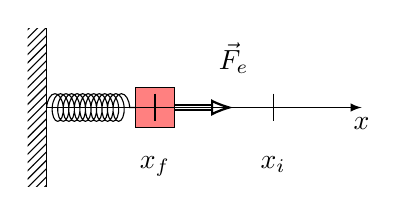
\begin{tikzpicture}
				\tikzstyle{ground}=[fill,pattern=north east lines,draw=none,minimum width=0.3,minimum height=0.6]

				\node (wall1) [ground, minimum height=2cm] {};
				\draw (wall1.north east) -- (wall1.south east);
				\node [draw, minimum width=0.5cm,minimum height=0.5cm, fill=red!50] (mass) at (1.5,0) {};
				\node (fix) at (0,0) {};
				\draw [
					snake=coil,
					segment amplitude=5pt,
					segment length=2pt
				] (wall1.east) -- (mass);
				\draw[-{Latex[open]}, thick, double distance=1pt] (mass) -- +(1,0) node[above=0.3cm] {$\vec F_e$};
				\draw[-latex] (wall1.east) -- +(4,0) node[below] {$x$};
				\node[mark size=5pt] at (mass) {\pgfuseplotmark{|}}; \node[below=0.5cm] at (mass) {$x_f$};
				\node[mark size=5pt] at ([xshift=1.5cm]mass) {\pgfuseplotmark{|}};\node[below=0.5cm] at ([xshift=1.5cm]mass) {$x_i$};
			\end{tikzpicture}
		\end{center}
	\end{minipage}\vspace*{1ex}

	The corresponding change in the elastic potential energy:
	\begin{equation*}
		\Delta U = -\int\limits_{x_i}^{x_f} (-kx) dx = \frac{kx_f^2}{2} - \frac{kx_i^2}{2}
	\end{equation*}
	To associate a potential energy value $U$ with the block at position $x$, we choose the reference configuration to be when the spring is at its relaxed length and the block is at $x_i = 0$. Then the elastic potential energy $U_i = 0$:
	\begin{equation*}
		\tcbhighmath[drop fuzzy shadow]{U = \frac{kx}{2}}
	\end{equation*}
\end{frame}
%=======================================================================================================

%=======================================================================================================
\begin{frame}{Conservation of Mechanical Energy}{}
	The mechanical energy $E$ of a system is the sum of its potential energy $U$ and
	the kinetic energy $K$ of the objects within it:
	\begin{equation*}
		\tcbhighmath[drop fuzzy shadow]{E = K + U}
	\end{equation*}
	\only<1>{%
		When a conservative force does work $W$ on an object within the system, that
		force transfers energy between kinetic energy $K$ of the object and potential
		energy $U$ of the system.}

	\only<2>{%
		From Work-kinetic energy theorem, the change $\Delta K$ in kinetic energy is
		\[
			\Delta K = W
		\]
		and from the relationship between the change $\Delta U$ in potential energy and work of conservative force
		\[
			-\Delta U = W
		\]
		Combining this equations, we find that}%
	\begin{equation*}
		\tcbhighmath[drop fuzzy shadow]{\Delta E = \Delta K + \Delta U = 0}
	\end{equation*}
	\only<3>{
		This result is called the \emph{principle of conservation of mechanical energy}
		\begin{boxedframe}
			In an isolated system where only conservative forces cause energy changes, the
			kinetic energy and potential energy can change, but their sum, the mechanical
			energy $E$ of the system, cannot change.
		\end{boxedframe}
	}
\end{frame}
%=======================================================================================================

%=======================================================================================================
\begin{frame}{Potential Energy and Conservative Force}{}
	Once again we consider a particle that is part of a system in which a conservative
	force acts. This time suppose that the particle is constrained to move along an
	$x$ axis while the conservative force does work on it.

	For one-dimensional motion, the work $W$ done by a force that acts on a particle
	as the particle moves through a distance $\Delta x$ is $F_x \Delta x$.
	From the relationship $W = -\Delta U$ we can then write:
	\begin{equation*}
		\Delta U(x) = - F_x\Delta x
	\end{equation*}
	Solving for $F(x)$ and passing to the differential limit yield:
	\begin{equation*}
		F_x = -\frac{dU}{dx}
	\end{equation*}
	In  3D case $F_x = -\frac{dU}{dx}, \, F_y = -\frac{dU}{dy} \, F_z = -\frac{dU}{dz}$ we can generalize:
	\begin{equation*}
		\vec F = -\left( \frac{dU}{dx} \vec i + \frac{dU}{dy} \vec j +\frac{dU}{dz} \vec k\right) = -\mathrm{grad} U
	\end{equation*}
\end{frame}
%=======================================================================================================

%=======================================================================================================
\begin{frame}{Gradient}{}
	\begin{columns}
		\begin{column}{0.7\linewidth}
			\begin{equation*}
				\vec F = -\left( \frac{dU}{dx} \vec i + \frac{dU}{dy} \vec j +\frac{dU}{dz} \vec k\right) = -\mathrm{grad} U
			\end{equation*}
			The meaning of a gradient becomes more obvious and
			descriptive as soon as we introduce the concept of an \emph{equipotential surface} at all of whose points \emph{the potential energy $U$
				has the same magnitude}.

			From equation follows  that \textbf{the vector
				$\vec F$ is normal to the equipotential surface at a given point}.

			Next, let us consider the displacement $d\vec r$ in the direction
			of decreasing $U$ values then the vector $\vec F$ is oriented in the  direction of decreasing $U$ values and vice versa, we may conclude that the gradient of $U$ is a vector oriented along a normal to an equipotential surface in the direction of increasing values of potential energy $U$.
		\end{column}
		\begin{column}{0.3\linewidth}
			\begin{center}
				\begin{tikzpicture}
					\path (0,0) +(70:4) arc (70:20:4)
					foreach \i in {0,2,...,8} {coordinate[pos=0.1*\i] (A\i)};

					\path (0,0) -- (-40:1)
					foreach \i  in {0,2,...,8} {coordinate[pos=0.1*\i] (B\i)};

					\foreach \i [count=\j] in {0,2,...,8} {
							\draw[thick, red, decoration={markings, mark=at position 0.5 with {
												\ifnum\i=4\node[pt=red] {};
													\coordinate (F);
												\fi
											}
									}, postaction={decorate}] (A\i) node[above,  black] {$U_{\j}$} to[bend right = 10pt] (B\i) ;
						}
					\draw[-latex, double] (F) -- +(140:1.5) node[above] {$\vec F$};
					\draw[-latex, double, red] (F) -- +(140+180:1.5) node[below] {$\mathrm{grad} U$};
				\end{tikzpicture}
				$\foreach \i  in {1,...,5} {
							\ifnum\i=1\relax\else <\fi U_\i
						}$
			\end{center}
		\end{column}
	\end{columns}


\end{frame}
%=======================================================================================================

%=======================================================================================================
\begin{frame}{The Potential Energy Curve}{}
	In the absence of a nonconservative force, the mechanical energy $E$ of a system has a constant value given by \begin{equation*}
		U(x) + K(x) = E = \mathrm{const}
	\end{equation*}

	Here $K(x)$ is the kinetic energy function kinetic energy as a function of the particle's location $x$. We may rewrite quation as
	\begin{equation*}
		K(x) = E - U(x)
	\end{equation*}
	Since $K(x)$ can never be negative (because $v^2$ is always positive), the particle can never move to the in region where $E < U$.
\end{frame}
%=======================================================================================================

%=======================================================================================================
\begin{frame}{The Potential Energy Curve}{}
	%================= Стилі для побудови графіків ====================
	\pgfplotsset{cartesian/.style={%
				% === Налаштування положення координатних осей ===
				%axis x line=center, % top, center, bottom
				%axis y line=center, % left, center, right
				axis lines = middle,
				axis line style={-stealth},
				% === Підпис координатних осей ===
				xlabel={$x$},
				ylabel={$U$, $E$},
				% === Положення підпису координатних осей ===
				xlabel style={below right},
				ylabel style={above right},
				% === Вибір підписів шкали для відображення ===
				xtick = \empty,
				ytick = \empty,
				% === Налаштування мінімальних та максимальних значень координат ===
				xmin = 0.5,
				xmax =  3,
				ymin = 0.6,
				ymax =  1,
				% === Налаштування розміру графіка ===
				%		width=1\linewidth,
				%		height=1\linewidth,
				% === Розширення границь осей ===
			}}
	\begin{columns}
		\begin{column}{0.5\linewidth}
			\only<1>{%
				Particle can move either in the region confined by the $x_1$ and $x_2$ coordinates (oscillation) or to the right of the $x_3$ coordinate.
				The particle cannot however pass from the first $ I $ region to the second $II$
				one (or vice versa) due to the potential barrier dividing these regions.}
			\only<2>{%
			A place where $K = 0$ (because $U = E$)  caled the \emph{turning point}, because particle change direction of motion in such point.

			$x_1$, $x_2$ and $x_3$ -- are \emph{turning points}.
			}
			\only<3>{%
			Region $I$ -- region of \emph{finite} motion;

			{\footnotesize 	When the particle reaches $x_1$, the force on the particle is positive (because the slope $dU/dx$ is negative). This means that the particle does not remain at $x_1$ but instead begins to move to the right, opposite its earlier motion. Also, when the particle reaches $x_2$, instead begins to move to the left.}
			}
			\only<4>{%
			Region $II$ -- region of \emph{infinite} motion;

			{\footnotesize 	When the particle reaches $x_3$, it begins to move to the right, opposite its earlier motion. But, when the particle heads to the right, it will continue indefinitely.}
			}
		\only<5>{
If the particle is located exactly at the minimum in point $x_\mathrm{stable}$, the force on it is zero, and the
		particle remains stationary. 
		If we push it slightly left or right, a restoring force
		appears that moves it back to $x_\mathrm{stable}$. A particle at such a position is said to be in \emph{stable
		equilibrium}. (A marble placed at the bottom of a hemispherical bowl is an example.)
		If we place the particle in the cup-like potential well centered at $x_{se}$, it is between two
		turning points.
	}
\only<6>{
 If the particle is located exactly at the minimum in point $x_\mathrm{unstable}$, the force on it is zero, and the
		particle remains stationary.  However, if it is displaced even slightly in either
		direction, a nonzero force pushes it farther in the same direction, and the particle
		continues to move. A particle at such a position is said to be in \emph{unstable equilibrium}.
		(A marble balanced on top of a bowling ball is an example.)	

	}
		\end{column}
		\begin{column}{0.5\linewidth}
			\begin{tikzpicture}[scale=0.8]
				\begin{axis}[cartesian, clip=false]
					\addplot[ultra thick, color=red, domain={0.65:3}, samples=500, name path global=GraphCurve] {8*0.95/(3*x-1)-3/x^2};
					\addplot [visible on=<1-4>, ultra thick, blue, thick, name path global=HorizontalLine]
					coordinates{(0.5,0.8) (3,0.8)} node[pos=0.8, above] {$E$};%
					\fill<1-4>
					[name intersections={of=GraphCurve and HorizontalLine, name=i, total=\t}]
					[red, opacity=1, every node/.style={above left, black, opacity=1}]
					\foreach \s in {1,...,\t}{(i-\s) coordinate (A\s) circle (2pt)
							node [above left] {\s}};
					\draw<1-4> (A1) -- ([yshift =-3cm]A1) node[below] {$x_1$};
					\draw<1-4> (A2) -- ([yshift =-3cm]A2) node[below] {$x_2$};
					\draw<1-4> (A3) -- ([yshift =-3cm]A3) node[below] {$x_3$};
					\node<1-4> at ([shift={(0.35cm,-1.5cm)}]A1) {$I$};
					\node<1-4> at ([shift={(0.5cm,-1.5cm)}]A3) {$II$};
					\draw<5>[dashed] (axis cs:0.5, 0.74) -- (axis cs:0.79, 0.74) node[below] {$x_\mathrm{stable}$};
					\draw<6>[dashed] (axis cs:0.5, .846) -- (axis cs:1.33, .846) node[above] {$x_\mathrm{unstable}$};
				\end{axis}
			\end{tikzpicture}
		\end{column}
	\end{columns}
\end{frame}
%=======================================================================================================

%=======================================================================================================
\begin{frame}{The Energy Conservation Law for a System}{}
Until now we confined ourselves to treating the behaviour of a single particle in terms of its energy. Now we shall pass over to a system of particles. That may be any object, gas, any device, the solar system, etc.

\end{frame}
%=======================================================================================================

\end{document}